\chapter{Информационная модель реактора} \label{model}

В данной главе будут рассмотрены устройство и особенности осуществления процесса перегрузки реактора на примере реактора БН-350.
Будет исследованы общие положения теории автоматов, а также будет предложена информационная модель реактора в терминах теории автоматов.

\section{Описательная информационная модель реактора} \label{BN}
\subsection{Общие сведения об устройстве реактора класса БН-350} 
Рассмотрим устройство энергетического реактора на быстрых нейтронах на примере установки БН-350.
Реактор БН-350 --- первый реактор на быстрых нейтронах энергетического  назначения (рис.~\ref{pic:basic-view}).
\begin{figure}[p]
\center{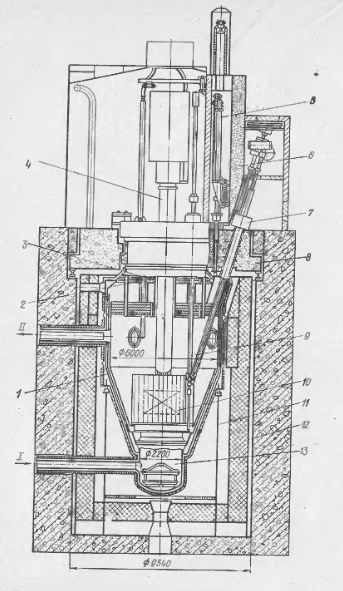
\includegraphics{basic-view}}
\caption[Общий вид реактора БН-350]{Общий вид реактора БН-350: 1 -- корпус реактора; 2 -- большая поворотная пробка; 3 -- малая поворотная пробка; 4 -- центральная поворотная колонка с механизмом СУЗ; 5 -- механизм передачи сборок; 6 -- передаточный бокс; 7 -- элеватор загрузки-выгрузки; 8 -- верхняя неподвижная защита; 9 -- механизм перегрузки; 10 -- активная зона; 11 -- опора реактора; 12 -- боковая защита; 13 -- напорная камера; I -- вход натрия; II -- выход натрия}
\label{pic:basic-view}
\end{figure}
В его конструкцию были заложены многие технические решения, выработанные на реакторе БОР-60, и впоследствии реализованные в конструкциях реакторов БН-600 и БН-800.
Внутри герметичного корпуса реактора, выполненного в виде бака переменного диаметра, расположены тепловыделяющие сборки (ТВС) активной зоны и боковой зоны воспроизводства, хранилище отработавших ТВС, отражатель нейтронов, механизмы системы перегрузки, стержни системы управления и защиты (СУЗ).
Натрий под давлением $~1$~МПа подводится от главных циркуляционных насосов (ГЦН) первого контура по шести напорным трубопроводам диаметром 500 мм в нижнюю часть корпуса реактора, образующую напорную камеру.
Сверху на камере закреплен напорный коллектор с установленными в нем ТВС.
В коллекторе поток теплоносителя распределяется по ТВС в соответствии с уровнем энерговыделения в них.
Он представляет собой прочную силовую конструкцию, воспринимающую весовую нагрузку от ТВС и других выемных частей реактора, а также внутренние давление теплоносителя.
Крепление коллектора к напорной камере допускает его извлечение и замену в случае необходимости.

Пройдя ТВС, нагретый натрий попадает в выходную смесительную камеру, откуда по шести сливным трубопроводам диаметром 600 мм отводится к промежуточным теплообменникам.

Активная зона набирается из шестигранных ТВС размером <<под ключ>> 96 мм. 
Каждая сборка содержит пучок гладкостержневых тепловыделяющих элементов (ТВЭЛов) диаметром 6,9 мм, расположенных с шагом 8 мм.
Топливо --- обогащенная двуокись урана.
Дистанцирование ТВЭЛов в пучке осуществляется проволокой, спирально навитой на оболочку ТВЭЛа.
Верхняя торцевая зона воспроизводства набирается из элементов увеличенного диаметра (12 мм) с двуокисью обедненного урана, установленных внутри сборки над пучком ТВЭЛов.
Гексагональная чехловая труба сборки несет давление теплоносителя, которое в нижней части значительно превышает давление в межкассетном пространстве реактора.
К чехлу сборки с обоих торцов приварены концевые детали цилиндрической формы: нижний хвостовик с боковыми отверстиями, через которые в ТВС поступает теплоноситель, и фигурная головка с выходными  окнами, предназначенная для захвата сборки механизмом перезагрузки.
Для уменьшения паразитных протечек натрия из напорного коллектора вдоль хвостовика сборки на нем предусмотрены лабиринтные уплотнения.
Зазор между ТВС принят минимальным (2 мм) исходя из условий нормального извлечения их при перезагрузке с учетом возможных при работе формоизменений.
Для пространственной фиксации сборок они дистанцируются с помощью выступов (<<платиков>>) в верхней части чехловых труб.

Часть гнезд в центральной области активной зоны занята органами СУЗ (рис.~\ref{pic:basic-grid})
\begin{figure}[ht]
\center{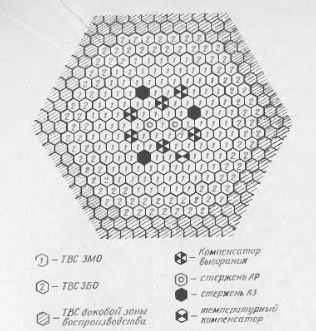
\includegraphics{basic-grid}}
\caption[Сетка СУЗ в реакторе БН-350]{Сетка СУЗ в реакторе БН-350: ЗМО -- зона малого обогащения, ЗБО -- зона большого обогащения}
\label{pic:basic-grid}
\end{figure}
Боковая зона воспроизводства общей толщиной 600 мм набрана из нескольких рядов ТВС, каждая из которых состоит из элементов диаметром 14,2 мм с двуокисью обедненного урана.
За внешним рядом сборок боковой зоны воспроизводства размещаются гнезда внутриреакторного хранилища, где отработавшие ТВС выдерживаются в течение интервала между перезагрузками реактора (2 месяца).
Необходимость выдержки сборок активной зоны перед выгрузкой из реактора обусловлена высоким уровнем остаточных тепловыделений в них.
В хранилище ТВС расхолаживаются теплоносителем, поступающим из напорного коллектора реактора.
После выдержки сборок значительно упрощается обращение с ними в тракте перегрузки.
Сборки боковой зоны воспроизводства имеют относительно низкое остаточное тепловыделение, поэтому предварительного охлаждения их перед выгрузкой не требуется.
Непосредственно за хранилищем устанавливается отражатель нейтронов из нескольких рядов стальных болванок с внешней конфигурацией ТВС (общая толщина 200 мм).

Натрий, заполняющий корпус реактора, образует свободный уровень, над которым находится аргоновая подушка.
Газовый объем служит для компенсации температурных расширений теплоносителя.
Вместе с тем он изолирует верхнюю часть реактора от горячего теплоносителя, выходящего из активной зоны, и защищает натрий от контакта с воздухом при случайной разгерметизации реактора.
Высота уровня над головками ТВС выбрана таким образом, чтобы транспортировка выгружаемых сборок проходила под слоем натрия, чем обеспечивается их надежное и эффективное охлаждение.
\cite{BH}

\subsection{Описание процесса планово-профилактического ремонта}\label{BN-PPM}

Рассмотрим процесс планово-профилактического ремонта для реактора БН-350.

Характерной особенностью конструкции реактора является то, что он не имеет съемной герметизирующей крышки, а перегрузка ТВС осуществляется без общего вскрытия корпуса герметичными дистанционно управляемыми механизмами под защитой инертного газа по закрытому тракту от реактора до внешнего хранилища.
Такое решение продиктовано специфическим требованием натриевой технологии --- недопустимостью контакта натрия с воздухом.
Сверху корпус реактора закрыт двумя многослойными плитами (<<пробками>>) верхней радиационной защиты.
Защитные пробки являются одновременно частью системы перегрузки реактора.
С их помощью осуществляются наведение внутриреакторного механизма перегрузки (ВМП) на ТВС, подлежащие перегрузке и перенос сборок внутри реактора. 
Эти операции выполняются совместным вращением обоих пробок --- большой, перекрывающей горловину реактора, и расположенной в ней эксцентрично малой пробки, в которую вмонтирован ВМП.
Обе пробки установлены на шаровых опорах, имеют по периферии зубчатый венец и электромеханические приводы, обеспечивающие их вращение по командам автоматизированной системы управления.
Поворотные пробки имеют значительный диаметр (большая пробка -- 4300 мм), поэтому создание надежного механического уплотнения по всему периметру, исключающего выход из реактора радиоактивного защитного газа, является весьма сложной технической задачей.
Благодаря небольшой разнице давлений между газовой полостью реактора и окружающей средой оказалось возможным выполнить уплотнение пробок в виде гидрозатвора: каждая пробка имеет цилиндрическую юбку, которая опущена в кольцевую ванну, заполненную тяжелой уплотняющей жидкостью, герметично связанную с корпусом реактора.
Уплотняющей средой в гидрозатворе служит сплав олова и висмута ($57\%$ Sn и $43\%$ Bi), имеющий плотность $~8,3\cdot10^3 \text{~кг/м}^3$ и температуру плавления $138^{\circ}\text{C}$.
При работе реактора сплав находится в твердом состоянии и вращение пробок невозможно.
Перед перегрузкой его расплавляют с помощью электронагревателей, вмонтированных в корпус гидрозатвора.

Перегрузка ТВС осуществляется на остановленном реакторе комплексом взаимодействующих механизмов в режиме автоматического управления.
Операции с ТВС внутри реактора (извлечение, перенос, установка) выполняются ВМП.
Он представляет собой прямую телескопическую штангу с захватным устройством и несколькими электромеханическими приводами.
После сцепления захвата с головкой перегружаемой сборки последняя втягивается внутрь направляющей трубы ВМП и в таком положении переносится вращением пробок в заданное место.
Перенос ТВС в направляющей трубе предохраняет сборку от раскачивания и случайных механических повреждений.
Выгрузка отработавших ТВС из реактора и загрузка свежих в реактор осуществляются через специальный перегрузочный патрубок небольшого диаметра в верхней части корпуса реактора с помощью двух механизмов: элеватора и механизма передачи сборок (МПС).
Элеватор представляет собой наклонный подъемник с цепным приводом и подвижной кареткой, в которую ВМП устанавливает перегружаемую сборку.
Движением каретки по наклонной направляющей сборка перемещается вверх под перегрузочный патрубок, в котором установлен МПС.
В точке встречи с механизмом передачи головка сборки выходит из-под уровня натрия в газовую полость реактора.
Это исключает погружение в натрий захвата МПС и повышает его надежность.
МПС втягивает сборку в герметичный передаточный бокс, установленный над перегрузочным патрубком, и транспортирует ее во внешние хранилище отработавших сборок.
Двигаясь в обратном направлении, МПС захватывает свежую ТВС, переносит ее к патрубку и устанавливает в каретку элеватора, которая опускает сборку в нижнее положение.
Отсюда она переносится с помощью ВМП в свободное гнездо активной зоны или боковой зоны воспроизводства. 
С учетом совмещения во времени операций, выполняемых различными механизмами перегрузочного комплекса, полный цикл перегрузки одного гнезда активной зоны (от извлечения отработавшей сборки до установки свежей) занимает около 50 минут.
\cite{BH}

\section{Формальное информационная модель реактора} \label{formal-model}
\subsection{Общие положения теории автоматов}\label{automata-theory}

Приведем общие понятия и положения теории автоматов, необходимые для построения формальной информационной модели реактора.

\begin{Def}
 Алфавитом $\Sigma$ называют некоторое непустое конечное множество символов.
\end{Def}

\begin{Def}
 Словом называют некоторую конечную (возможно, пустую) последовательность символов алфавита: $\omega = \sigma_1\sigma_2\dots\sigma_l$. 
 Количество символов в слове (число $l$) называют длиной слова. 
 Пустое слово принято обозначать $\varepsilon$.
\end{Def}

\begin{Def}
 Детерминированным конечным автоматом (ДКА) называется пятерка (кортеж) $A = \langle Q, \Sigma, \delta, q_0, F  \rangle$, где:
 \begin{itemize}
  \item [-] $Q$ --- конечное множество состояний;
  \item [-] $\Sigma$ --- алфавит;
  \item [-] $\delta : Q \times \Sigma \rightarrow Q$ --- функция переходов;
  \item [-] $q_0 \in Q$ --- начальное состояние;
  \item [-] $F \subseteq Q$ --- множество терминальных (конечных) состояний.
 \end{itemize}
\end{Def}

Обработка слова $\omega = \sigma_1\sigma_2\dots\sigma_l$ ДКА $A$ происходит следующим образом. 
Сначала автомат $A$ находится в стартовом состоянии $q_0$. 
Затем на каждом шаге обработки автомат считывает очередной символ $sigma_i$ слова $\omega$ и переходит из своего текущего состояния $q$ в состояние $\delta(q; \omega_i)$. 
К моменту, когда все символы входного слова $\omega$ обработаны, автомат находится в некотором состоянии $p$. Говорят, что автомат A принимает слово $\omega$, если $p \in F$, и не принимает в обратном случае.\cite{TA-defs}

Определение ДКА как пятерки объектов с детальным описанием функций переходов слишком сухое и неудобочитаемое.
Существует два более удобных способа описания автоматов.
\begin{enumerate}
 \item \textit{Диаграмма переходов}, которая представляет собой граф.
 \item \textit{Таблица переходов}, дающая табличное представление функции $\delta$.
 Из нее очевидны состояния и входной алфавит.
\end{enumerate}

\begin{figure}[ht]
\center{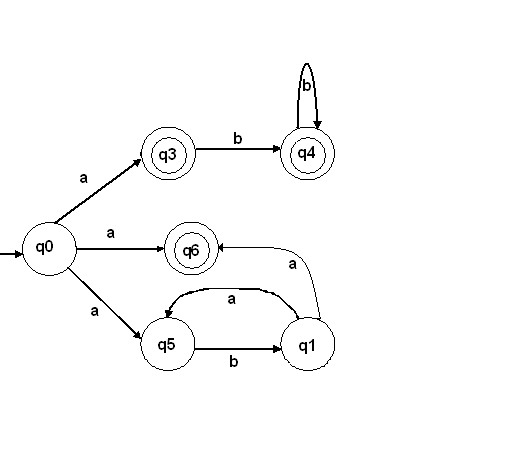
\includegraphics[width=0.6\linewidth]{auto.jpg}}
\caption[Пример диаграммы перехода конечного автомата]{Пример диаграммы перехода конечного автомата}
\label{pic:auto}
\end{figure}

\textit{Диаграмма переходов} (см. рис.~\ref{pic:auto}) для ДКА вида $A = \langle Q, \Sigma, \delta, q_0, F  \rangle$ есть граф, определяемый следующим образом:
\begin{itemize}
 \item [a)] всякому состоянию из $Q$ соответствует некоторая вершина;
 \item [б)] пусть $\delta(q, a) = p$ для некоторого состояния $q$ из $Q$ и входного символа $a$ из $\Sigma$.
 Тогда диаграмма переходов должна содержать дугу из вершины $q$ в вершину $p$, отмеченную $a$.
 Если существует несколько входных символов, переводящих автомат $A$ из состояния $q$ в состояние $p$, то диаграмма переходов может содержать одну дугу, отмеченную списком этих символов;
 \item [в)] диаграмма содержит стрелку в начальное состояние, отмеченную как \textit{Начало}.
 Эта стрелка не выходит не из какого состояния;
 \item [г)] вершины, соответствующие допускающим состояниям (состояниям из $F$), отмечаются двойным кружком.
 Состояния, не принадлежащие $F$, изображаются простым (одинарным) кружком.
\end{itemize}


\textit{Таблица переходов} представляет собой обычное табличное представление функции, подобной $\delta$, которая двум значениям ставит в соответствие одно значение.
Строки таблицы соответствуют состояниям, а столбцы --- входным символам.
На пересечении строки, соответствующей состоянию $q$, и столбца, соответствующего символу $a$, находится состояние $\delta(q, a)$. 
\cite{Intro-TA}

\begin{Def}
Автомат называется \textit{полностью определенным} или \textit{полным}, если $D_\delta = Q \times \Sigma$.
Иными словами, для любого начального состояния и любой входной последовательности (в пределах алфавита $\Sigma$) однозначно определена выходная последовательность.
\end{Def}

\begin{Def}
Автомат называется \textit{частично определенным} или \textit{частичным}, если функция $\delta$ определена не для всех пар $(q, a) \in Q \times \Sigma$. 
\end{Def}

В табличном задании таких автоматов на месте неопределенных состояний и выходных сигналов ставится прочерк. 
На графе автомата неопределенному состоянию можно поставить в соответствие дополнительную вершину.

Неопределенное состояние автомата называется граничным. 
Дальнейшее поведение автомата, попавшего в граничное состояние, не определяется. 
Выходная последовательность, содержащая неопределенные сигналы, называется частичной.
Заметим, что модель частичного автомата является более абстрактной, чем модель полного автомата: она задает целое множество дискретных устройств. \cite{TA-Syntes}



Под \textit{композицией элементарных автоматов} в общем случае понимается следующее.
Пусть заданы элементарные автоматы $A_1, A_2, \dots, A_k$.
Произведем объединение элементарных автоматов в систему совместно работающих автоматов. 
Введем в рассмотрение некоторое конечное множество узлов, называемых внешними выходными узлами. 
Эти узлы отличаются от узлов рассматриваемых элементарных автоматов, которые носят название внутренних.
Композиция автомата состоит в том, что в полученной системе элементарных автоматов $A_1, A_2, \dots, A_k$ и внешних узлов производится отождествление некоторых узлов (как внешних так и внутренних). 

С точки зрения совместной работы системы автоматов смысл операции отождествления узлов состоит в том, что элементарный сигнал, попадающий на один из узлов, входящих в множество отождествляемых между собой узлов, попадает тем самым на все узлы этого множества. 
После проведенных отождествлений узлов система автоматов превращается в так называемую схему (сеть) автоматов.
Будем считать, что автоматы, входящие в систему автоматов, работают совместно, если в каждый момент автоматного времени на все внешние входные узлы подается набор входных сигналов (структурный входной сигнал схемы) и со всех внешних выходных узлов снимается набор выходных сигналов (структурный выходной сигнал). 
Следует заметить, что при построении схемы автоматов должны выполняться условия корректности. 
\cite{TA-Lupal}
		
\subsection{Описание реактора в терминах теории автоматов}\label{TA-model}

Исходя из положений, представленных в разделах \ref{BN} и \ref{automata-theory}, представим реактор как композицию конечных детерминированных автоматов.

Пусть реактор состоит из $k$ структурных элементов, каждый из которых можно представить как конечный детерминированный автомат.
Таким образом $i-$й структурный элемент реактора описывается кортежем $A_i = \langle Q^i, \Sigma^i, \delta^i, q_0^i, F^i  \rangle$. 

Тогда реактор можно представить следующим кортежем $A = \langle Q, \Sigma, \delta, q_0, F  \rangle$, где
\begin{itemize}
 \item [-] $Q = \cup_{i=0}^n Q^i$;
 \item [-] $\Sigma = \cup_{i=0}^n \Sigma^i$;
 \item [-] $\delta = f (q, a)$;
 \item [-] $q_0 = \cup_{i=0}^n q_0^i$;
 \item [-] $F = \cap_{i=0}^n F^i$.
\end{itemize}

Рассмотрим данную модель на примере фиктивного реактора.
Пусть реактор имеет следующую конфигурацию активной зоны (см. рис.~\ref{pic:fict-grid}).
Ячейки А1, Б1, В1, Г1, Д1, Е1 предназначены для организации внутриреакторного хранилища отработавших ТВС, 
ячейки А2, Б2, В2, Г2, Д2, Е2 содержат сборки для организации боковой зоны воспроизводства, ячейки А3, Б3, В3, Г3, Д3, Е3 содержат сборки активной зоны реактора и ячейка А4 содержит механизм автоматического регулирования реактора.
\begin{figure}[ht]
\center{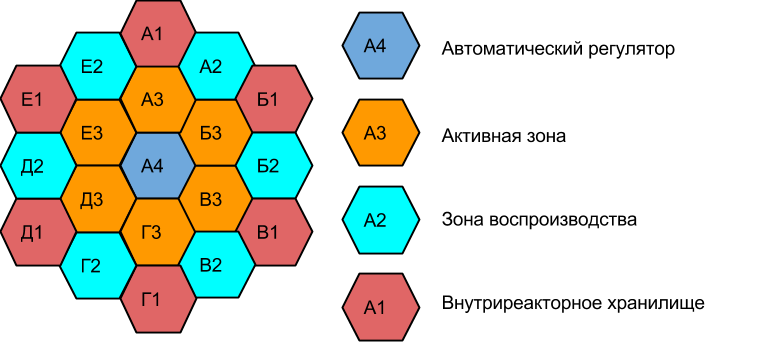
\includegraphics[width=\linewidth]{fict-grid}}
\caption[Конфигурация активной зоны фиктивного реактора]{Конфигурация активной зоны фиктивного реактора: A1 -- внутриреакторное хранилище, А2 -- зона воспроизводства, А3 --- активная зона, А4 --- автоматический регулятор}
\label{pic:fict-grid}
\end{figure}

Фиктивный реактор имеет механизм перегрузки, аналогичный описанному в \ref{BN-PPM}.
Большая поворотная пробка имеет 6 положений, которые соответствуют букве в названии ячейки, малая поворотная пробка - 4 положения, которые соответствуют цифре в названии ячейки.

Перед началом планово-профилактического ремонта поворотные пробки находятся в положении А1, активная зона и зоны воспроизводства  полностью заполнены, внутриреакторное хранилище пусто, частично или полностью заполнено.
Некоторые ТВС активной зоны и зоны воспроизводства, а также все ТВС из внутриреакторного хранилищ помечены как требующие перезагрузки. 
После планово-профилактического ремонта поворотные пробки находятся в положении А1, активная зона и зоны воспроизводства  полностью заполнены, внутриреакторное хранилище пусто, частично или полностью заполнено.
Все ТВС активной зоны и зоны воспроизводства, а также все ТВС из внутриреакторного хранилищ помечены как не требующие перезагрузки. 

Разделим реактор на следующие структурные компоненты: тепловыделяющие сборки с обогащенным ураном, тепловыделяющие сборки с обедненным ураном, гнезда внутриреакторного хранилища, гнезда зоны воспроизводства, гнезда активной зоны, большая поворотная пробка, малая поворотная пробка, перегрузочный механизм.
Рассмотрим отдельные структурные компоненты реактора как автоматы.

\textbf{Тепловыделяющие сборки с обогащенным ураном}:
\begin{itemize}
 \item [-] $Q = \{\text{В активную зону}, \text{Во внутриреакторное хранилище}, \text{Во внешнее хранилище}, \\ \text{Обслуживание завершено}\}$;
 \item [-] $\Sigma = \{\text{Обслужить}\}$;
 \item [-] $\delta = f (q, a)$, где $f$ соответствует таблице~\ref{tab:EFuel};
 \item [-] $q_0 \in \{\text{В активную зону}, \text{Во внутриреакторное хранилище}, \text{Во внешнее хранилище}, \\ \text{Обслуживание завершено}\}$;
 \item [-] $F = \{\text{Обслуживание завершено}\}$.
\end{itemize}

\begin{table} [htbp]
  \centering
  \parbox{15cm}{\caption{Таблица переходов автомата <<Тепловыделяющая сборка с обогащенным ураном>>}\label{tab:EFuel}}
  \begin{center}
  \begin{tabular}{| c | c |}
  \hline
  $q_i \diagdown \sigma_j$& Обслужить \\
  \hline
  В активную зону & Обслуживание завершено\\
  \hline
  Во внутриреакторное хранилище & Обслуживание завершено\\
  \hline
  Во внешнее хранилище& Обслуживание завершено\\
  \hline
  Обслуживание завершено & ---\\
  \hline
  \end{tabular}
  \end{center}
\end{table}

\textbf{Тепловыделяющие сборки с обедненным ураном}:
\begin{itemize}
 \item [-] $Q = \{\text{В зону воспроизводства}, \text{Во внешнее хранилище}, \text{Обслуживание завершено}\}$;
 \item [-] $\Sigma = \{\text{Обслужить}\}$;
 \item [-] $\delta = f (q, a)$, где $f$ соответствует таблице~\ref{tab:DFuel};
 \item [-] $q_0 \in \{\text{В зону воспроизводства}, \text{Во внешнее хранилище}, \text{Обслуживание завершено}\}$;
 \item [-] $F = \{\text{Обслуживание завершено}\}$.
\end{itemize}

\begin{table} [htbp]
  \centering
  \parbox{15cm}{\caption{Таблица переходов автомата <<Тепловыделяющая сборка с обедненным ураном>>}\label{tab:DFuel}}
  \begin{center}
  \begin{tabular}{| c | c |}
  \hline
  $q_i \diagdown \sigma_j$& Обслужить \\
  \hline
  В зону воспроизводства & Обслуживание завершено\\
  \hline
  Во внешнее хранилище& Обслуживание завершено\\
  \hline
  Обслуживание завершено & ---\\
  \hline
  \end{tabular}
  \end{center}
\end{table}

\textbf{Гнезда внутриреакторного хранилища}:
\begin{itemize}
 \item [-] $Q =  A_{ef} \cup \varnothing$, где $A_{ef}$ -- множество автоматов <<Тепловыделяющая сборка с обогащенным ураном>>;
 \item [-] $\Sigma =  A_{ef} \cup \varnothing$, где $A_{ef}$ -- множество автоматов <<Тепловыделяющая сборка с обогащенным ураном>>;
 \item [-] $\delta = f (q, a)$, где $f$ соответствует таблице~\ref{tab:PlaceIn};
 \item [-] $q_0 \in Q$;
 \item [-] $F \in Q$.
\end{itemize}

\begin{table} [htbp]
  \centering
  \parbox{15cm}{\caption{Таблица переходов автомата <<Гнездо внутриреакторного хранилища>>}\label{tab:PlaceIn}}
  \begin{center}
  \begin{tabular}{| c | c | c |}
  \hline
  $q_i \diagdown \sigma_j$& $a_{ef}$ & $\varnothing$ \\
  \hline
  $a_{ef}$&  --- & $\varnothing$\\
  \hline
  $\varnothing$ & $a_{ef}$ & ---\\
  \hline
  \end{tabular}
  \end{center}
\end{table}

\textbf{Гнезда зоны воспроизводства}:
\begin{itemize}
 \item [-] $Q =  A_{uf} \cup \varnothing$, где $A_{uf}$ -- множество автоматов <<Тепловыделяющая сборка с обедненным ураном>>;
 \item [-] $\Sigma =  A_{uf} \cup \varnothing$, где $A_{uf}$ -- множество автоматов <<Тепловыделяющая сборка с обедненным ураном>>;
 \item [-] $\delta = f (q, a)$, где $f$ соответствует таблице~\ref{tab:PlaceRes};
 \item [-] $q_0 \in A_{uf} $;
 \item [-] $F \in A_{uf} $.
\end{itemize}

\begin{table} [htbp]
  \centering
  \parbox{15cm}{\caption{Таблица переходов автомата <<Гнездо зоны воспроизводства>>}\label{tab:PlaceRes}}
  \begin{center}
  \begin{tabular}{| c | c | c |}
  \hline
  $q_i \diagdown \sigma_j$& $a_{uf}$ & $\varnothing$ \\
  \hline
  $a_{uf}$&  --- & $\varnothing$\\
  \hline
  $\varnothing$ & $a_{uf}$ & ---\\
  \hline
  \end{tabular}
  \end{center}
\end{table}

\textbf{Гнезда активной зоны}:
\begin{itemize}
 \item [-] $Q =  A_{ef} \cup \varnothing$, где $A_{ef}$ -- множество автоматов <<Тепловыделяющая сборка с обогащенным ураном>>;
 \item [-] $\Sigma =  A_{ef} \cup \varnothing$, где $A_{ef}$ -- множество автоматов <<Тепловыделяющая сборка с обогащенным ураном>>;
 \item [-] $\delta = f (q, a)$, где $f$ соответствует таблице~\ref{tab:PlaceAct};
 \item [-] $q_0 \in A_{ef} $;
 \item [-] $F \in A_{ef} $.
\end{itemize}

\begin{table} [htbp]
  \centering
  \parbox{15cm}{\caption{Таблица переходов автомата <<Гнездо активной зоны>>}\label{tab:PlaceAct}}
  \begin{center}
  \begin{tabular}{| c | c | c |}
  \hline
  $q_i \diagdown \sigma_j$& $a_{ef}$ & $\varnothing$ \\
  \hline
  $a_{ef}$&  --- & $\varnothing$\\
  \hline
  $\varnothing$ & $a_{ef}$ & ---\\
  \hline
  \end{tabular}
  \end{center}
\end{table}


\textbf{Большая поворотная пробка}:
\begin{itemize}
 \item [-] $Q = \{\text{А}, \text{Б}, \text{В}, \text{Г}, \text{Д}, \text{Е}\}$;
 \item [-] $\Sigma = \{\text{влево}, \text{вправо}\}$;
 \item [-] $\delta = f (q, a)$, где $f$ соответствует таблице~\ref{tab:BP};
 \item [-] $q_0 = \text{А}$;
 \item [-] $F = \text{А}$.
\end{itemize}

\begin{table} [htbp]
  \centering
  \parbox{15cm}{\caption{Таблица переходов автомата <<Большая поворотная пробка>>}\label{tab:BP}}
  \begin{center}
  \begin{tabular}{| c | c | c |}
  \hline
  $q_i \diagdown \sigma_j$& влево & вправо \\
  \hline
  А & Е & Б\\
  \hline
  Б & А & В\\
  \hline
  В & Б & Г\\
  \hline
  Г & В & Д\\
  \hline
  Д & Г & Е\\
  \hline
  Е & Д & А\\
  \hline
  \end{tabular}
  \end{center}
\end{table}



\textbf{Малая поворотная пробка}:
\begin{itemize}
 \item [-] $Q = \{1, 2, 3, 4\}$;
 \item [-] $\Sigma = \{\langle \text{влево}, q_{bp}\rangle, \langle \text{вправо}, q_{bp}\rangle\}$, где $q_{bp}$ -- текущее состояние автомата <<Большая поворотная пробка>>;
 \item [-] $\delta = f (q, a)$, где $f$ соответствует таблице~\ref{tab:SP};
 \item [-] $q_0 = 1$;
 \item [-] $F = 1$.
\end{itemize}

\begin{table} [htbp]
  \centering
  \parbox{15cm}{\caption{Таблица переходов автомата <<Малая поворотная пробка>>}\label{tab:SP}}
  \begin{center}
  \begin{tabular}{| c | c | c | c | c |}
  \hline
  $q_i \diagdown \sigma_j$ & $\langle \text{влево}, \text{А} \rangle$ & $\langle \text{вправо}, \text{А}\rangle$ & $\langle \text{влево}, \overline{\text{А}}\rangle$ & $\langle \text{вправо}, \overline{\text{А}}\rangle$\\
  \hline
  1 &4&2&3&2\\
  \hline
  2 &1&3&1&3\\
  \hline
  3 &2&4&2&1\\
  \hline
  4 &3&1&-&-\\
  \hline
  \end{tabular}
  \end{center}
\end{table}

\textbf{Перегрузочный механизм}:
Рассмотрим перегрузочный механизм как совокупность следующих автоматов: большая поворотная пробка, малая поворотная пробка, определитель типа гнезда, селектор гнезда, перегрузочный механизм.

\textit{Определитель типа гнезда}:
\begin{itemize}
 \item [-] $Q = \{\text{Внутриреакторное хранилище}, \text{Зона воспроизводства}, \text{Активная зона},\\
 \text{Автоматический регулятор}\}$;
 \item [-] $\Sigma = \{1, 2, 3, 4\}$;
 \item [-] $\delta = f (q, a)$, где $f$ соответствует таблице~\ref{tab:Determinator};
 \item [-] $q_0 = \text{Внутриреакторное хранилище}$;
 \item [-] $F = \text{Внутриреакторное хранилище}$.
\end{itemize}
\begin{table} [htbp]
  \centering
  \parbox{15cm}{\caption[Таблица переходов автомата <<Определитель типа гнезда>>]{Таблица переходов автомата <<Определитель типа гнезда>>: ВХ -- Внутриреакторное хранилище; ЗВ -- Зона воспроизводства; АЗ -- Активная зона; АР -- Автоматический регулятор.}\label{tab:Determinator}}
  \begin{center}
  \begin{tabular}{| c | c | c | c | c |}
  \hline
  $q_i \diagdown \sigma_j$ & 1 & 2 & 3& 4\\
  \hline
  ВХ& ВХ& ЗВ& АЗ& АР\\
  \hline
  ЗВ& ВХ& ЗВ& АЗ& АР\\
  \hline
  АЗ& ВХ& ЗВ& АЗ& АР\\
  \hline
  АР& ВХ& ЗВ& АЗ& АР\\
  \hline
  \end{tabular}
  \end{center}
\end{table}

\textit{Селектор гнезда}:
\begin{itemize}
 \item [-] $Q = Q_{\text{гнезда}}$;
 \item [-] $\Sigma = \langle Q_{\text{A1}},\dots, Q_{\text{Е3}}, Q_{bp}, Q_{lp}\rangle$;
 \item [-] $\delta = f (q, a)$, где $f$ соответствует таблице~\ref{tab:Selector};
 \item [-] $q_0 = Q_{\text{A1}}$;
 \item [-] $F = Q_{\text{A1}}$.
\end{itemize}

\begin{table} [htbp]
  \centering
  \parbox{15cm}{\caption{Таблица переходов автомата <<Селектор гнезда>>.}\label{tab:Selector}}
  \begin{center}
  \begin{tabular}{| c | c | c | c |}
  \hline
  $q_i \diagdown \sigma_j$ & $\langle q_{\text{A1}},\dots, q_{\text{Е3}}, \text{A}, 1\rangle$ & $\cdots$ & 
  $\langle q_{\text{A1}},\dots, q_{\text{Е3}}, \text{Е}, 3\rangle$\\
  \hline
  $\forall q \in Q$& $q_{\text{A1}}$ & $\cdots$ & $q_{\text{Е3}}$\\
  \hline
  \end{tabular}
  \end{center}
\end{table}

\textit{Перегрузочный механизм}:
\begin{itemize}
 \item [-] $Q = A_{\text{ТВС}} \cup \varnothing$;
 \item [-] $\Sigma = \langle Q_{\text{Селектора}},\dots, Q_{\text{Определителя}}, \{\text{извлечь}, \text{установить}, \text{во внешнее хранилище},\\ \text{из внешнего хранилища}\}\rangle$;
 \item [-] $\delta = f (q, a)$, где $f$ соответствует таблице~\ref{tab:Elevator};
 \item [-] $q_0 = \varnothing$;
 \item [-] $F = \varnothing$.
\end{itemize}

\begin{table} [htbp]
  \centering
  \parbox{15cm}{\caption[Таблица переходов автомата <<Перегрузочный механизм>>]{Таблица переходов автомата <<Перегрузочный механизм>>: ВХ -- Внутриреакторное хранилище; ВнешХ -- Внешнее хранилище; ЗВ -- Зона воспроизводства; АЗ -- Активная зона; АР -- Автоматический регулятор.}\label{tab:Elevator}}
  \begin{center}
  \begin{tabular}{| c | c | c | c | c | c | }
  \hline
  $\sigma_j \diagdown q_i$ & $\varnothing$ & В АЗ & Во ВХ & Во внешХ & В ЗВ\\
  \hline
  $\langle \varnothing, \text{АЗ}, \text{извлечь}\rangle$&---&---&---&---&---\\
  \hline
  $\langle \varnothing, \text{АЗ}, \text{установить}\rangle$&---&$\varnothing$&---&---&---\\
  \hline
  $\langle \varnothing, \text{АЗ}, \text{во внешнее хранилище}\rangle$&---&---&---&---&---\\
  \hline
  $\langle \varnothing, \text{АЗ}, \text{из внешнего хранилища}\rangle$&$A_{\text{ТВС}}$&---&---&---&---\\
  \hline
  $\cdots$&$\cdots$&$\cdots$&$\cdots$&$\cdots$&$\cdots$\\
  \hline
  $\langle \text{В ЗВ}, \text{ВХ}, \text{из внешнего хранилища}\rangle$&---&---&---&---&---\\
  \hline
  \end{tabular}
  \end{center}
\end{table}

Рассмотрев отдельные автоматы, моделирующие поведение структурных элементов реактора, рассмотрим композицию этих автоматов (ТА-модель).
Согласно описанию фиктивного реактора, приведенного выше (см. рис.~\ref{pic:fict-grid}), ТА-модель реактора состоит из $6-12$ ТА-моделей тепловыделяющих сборок с обогащенным ураном, $6$ ТА-моделей тепловыделяющих сборок с обедненным ураном, $6$ ТА-моделей гнезд активной зоны, $6$ ТА-моделей гнезд зоны воспроизводства, $6$ ТА-моделей гнезд внутриреакторного хранилища, ТА-модели большой поворотной пробки, ТА-модели малой поворотной пробки, ТА-модели селектора гнезд, ТА-модели определителя типа гнезда и ТА-модели перегрузочного механизма.    

Выходы ТА-моделей ТВС с обогащенным ураном являются входными символами для ТА-моделей гнезд активной зоны и ТА-моделей гнезд внутриреакторного хранилища. 
Выходы ТА-моделей ТВС с обедненным ураном являются входными символами для ТА-модели гнезд зоны воспроизводства. 
Выходы ТА-моделей гнезд реактора являются входными символами ТА-модели селектора гнезд. 
Выход ТА-модели большой поворотной пробки является входным символом для ТА-моделей малой поворотной пробки, селектора гнезд и определителя типа гнезд.
Выход ТА-модели малой поворотной пробки является входным символом для ТА-модели селектора гнезд и определителя типа гнезд.
Выходы ТА-моделей селектора гнезд и определителя типа гнезд являются входными символами для ТА-модели перегрузочного механизма.
Композиционная схема ТА-модели фиктивного реактора представлена на рисунке~\ref{pic:fict-composition}.

\begin{figure}[ht]
\center{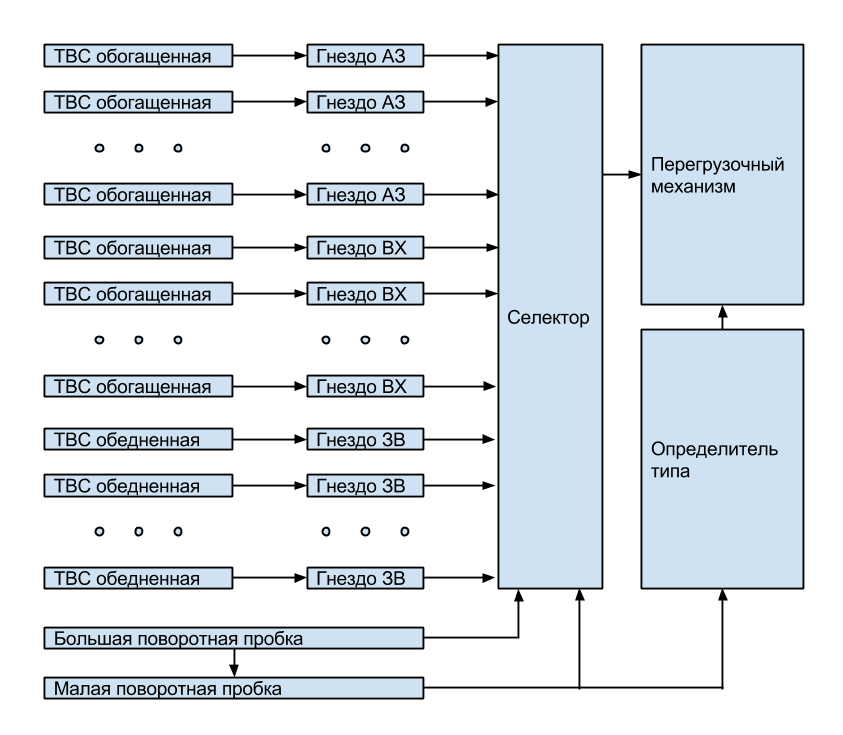
\includegraphics[width=\linewidth]{fict-composition}}
\caption[Композиционная схема автоматов модели фиктивного реактора]{Композиционная схема автоматов модели фиктивного реактора: ТВС -- тепловыделющая сборка, ВХ -- Внутриреакторное хранилище; ЗВ -- Зона воспроизводства; АЗ -- Активная зона.}
\label{pic:fict-composition}
\end{figure}

Исходя из описанного выше представим модель фиктивного реактора в общем виде следующим образом:
\begin{itemize}
 \item [-] $Q = \langle Q_{\text{ТВС 1}}, \dots, Q_{\text{ТВС 18}}, Q_{\text{A1}},\dots, Q_{\text{Е3}}, Q_{bp}, Q_{lp}, Q_{\text{перегрузочного механизма}} \rangle$;
 \item [-] $\Sigma = \{\text{извлечь}, \text{установить}, \text{во внешнее хранилище}, \text{из внешнего хранилища},\\ \text{БПП влево}, \text{БПП вправо}, \text{МПП влево}, \text{МПП вправо}\}$;
 \item [-] $\delta = \delta_{\text{ТВС 1}} \cdot \dots \cdot  \delta_{\text{ТВС 18}} \cdot  \delta_{\text{A1}} \cdot \dots \cdot \delta_{\text{Е3}} \cdot  \delta_{bp} \cdot  \delta_{lp} \cdot \delta_{\text{перегрузочного механизма}}$;
 \item [-] $q_0 = \langle q_{\text{ТВС 1}}, \dots, q_{\text{ТВС 18}}, q_{\text{A1}},\dots, q_{\text{Е3}}, q_{bp}, q_{lp}, q_{\text{перегрузочного механизма}} \rangle$;
 \item [-] $F = \langle F_{\text{ТВС 1}}, \dots, F_{\text{ТВС 18}}, F_{\text{A1}},\dots, F_{\text{Е3}}, F_{bp}, F_{lp}, F_{\text{перегрузочного механизма}} \rangle$.
\end{itemize}

Таким образом, были рассмотрены устройство и особенности осуществления процесса перегрузки реактора на примере реактора БН-350.
Будет исследованы общие положения теории автоматов, а также будет предложена информационная модель реактора в терминах теории автоматов (ТА-модель) для фиктивного реактора.




\clearpage